\section{设计过程}
\subsection{设计流水账}

\begin{enumerate}
    \item 2022年12月22日19:00$\sim$凌晨1点:两人一起配置环境(Vivado2019.2,Verilator,gtkwave,实验包),复习Vivado的使用,学习Verilator gtkwave等新工具的使用,结果是学会了。
    \item 2022年12月23日15:00$\sim$18:00,两人一起修改ALU架构(去掉了aluop),重写原来的12条指令,结果是改好了。
    \item 2022年12月24日15:00$\sim$18:00,\stunameb 添加8条逻辑指令和6条移位运算指令,\stunamea 设计HILO方案,结果是添加好了,并且设计好了。
    \item 2022年12月25日
    \begin{enumerate}[(1)]
        \item 14:00$\sim$19:00,两人一起添加hilo和14条算术运算指令。
        \item 20:00$\sim$24:00,两人一起添加12条转移指令。
    \end{enumerate}
    结果是添加成功。
    \item 2022年12月26日
    \begin{enumerate}[(1)]
        \item 10:00$\sim$12:00,两人一起设计访存指令方案。
        \item 14:00$\sim$15:00,两人一起添加访存指令。
    \end{enumerate}
    结果是该日,52条指令完成,但没有通过功能测试。
    \item 2022年12月28日20:00$\sim$凌晨1点,两人一起连接SRAMSOC,并debug前64个功能测试,最终通过。
    \item 2022年12月30日
    \begin{enumerate}[(1)]
        \item 9:00$\sim$15:00,两人一起完成52条指令SRAMSOC并各自上板成功。
        \item 15:00$\sim$19:00,两人一起完成57条指令功能测试通过并各自上板成功。
    \end{enumerate}
    \item 2022年12月31日
    \begin{enumerate}[(1)]
        \item 9:00$\sim$12:00,两人一起讨论研究AXI和Cache,结果是讨论了一个方案出来。
        \item 15:00$\sim$18:00,两人一起做系统结构实验(提前把硬件综合的Cache准备好),结果是完成了系统结构的实验。
    \end{enumerate}
    \item 2023年1月1日(元旦)
    \begin{enumerate}[(1)]
        \item 14:00$\sim$18:00,两人一起连接AXI和Cache,写转接桥,修改mycpu\_top,并debug,结果是没debug完。
        \item 20:00$\sim$24:00,两人继续一起debug,结果是AXI和Cache功能测试通过,性能测试通过。
    \end{enumerate}
    \item 2023年1月2日
    \begin{enumerate}[(1)]
        \item 9:30$\sim$11:00,两人一起写报告,结果是没写完。
        \item 14:00$\sim$17:00,两人各自完成一些模块的通路图,写报告,结果是通路图画完了,报告没写完。
        \item 19:00$\sim$22:00,写报告,结果是写完了。
    \end{enumerate}
    \item 2023年1月3日19:00$\sim$24:00,发现1月2日半场开香槟,之前没测perfdiff,现在发现perfdiff炸了,debug一晚上未果,确定了是dcache带来的问题。
    \item 2023年1月4日22:00$\sim$凌晨2点,发现perdiff过不了是因为sramto类sram转接口读取的时候有非法组合,改了之后就过了perfdiff,但此时性能低于10分,为了让性能高于10分,写了一个双周期乘法器,把性能提高到了11分。同时尝试了用系统结构实验的四路组相联cache和普通写回cache,因不同的问题而放弃。
    \item 2023年1月6日15:00$\sim$17:00,补充报告。
\end{enumerate}

\subsection{错误记录}



\subsubsection{错误1}
\begin{enumerate}[(1)]
    \item 错误现象:bgtz触发了不该触发的异常
    \item 分析定位过程:根据波形图,能看到bgtz指令发生了异常,仔细检查后发现是bgtz被aludec译码出来的结果是有符号减法,而触发了overflow。
    \item 错误原因:aludec译码错了,bgtz被aludec译码出来的结果是有符号减法,而触发了overflow。
    \item 修正效果:将aludec译码bgtz改为subu(无符号)。
    \item 归纳总结:修改文件后,没有全面考虑,导致某些信号没有修改到。
\end{enumerate}

\subsubsection{错误2}
\begin{enumerate}[(1)]
    \item 错误现象:div算出来的结果,与正确结果互为相反数。
    \item 分析定位过程:通过波形图可以发现div计算的过程中,前面的部分都是正确的,直到最后一个周期的时候,原本的正确答案突然变成负的正确答案。仔细查看div的写法,我们发现在最后一个周期的时候,会根据op\_data的值改变得到的结果,而op\_data在整个过程中发生了变化,而op\_data是alu的srca2E传进来的,因此是srca2E出了问题。
    \item 错误原因:刚开始的srca2E是M阶段前推过来的,但是我们的div只stall了前三个阶段,因此,在M阶段的指令流走了之后,前推也没了。虽然M阶段的那条指令已经写入了regfile,但是由于stall的存在,不能把正确的值读到E阶段。(当时讨论的截图如下)
    \begin{figure}[H]
        \centering
        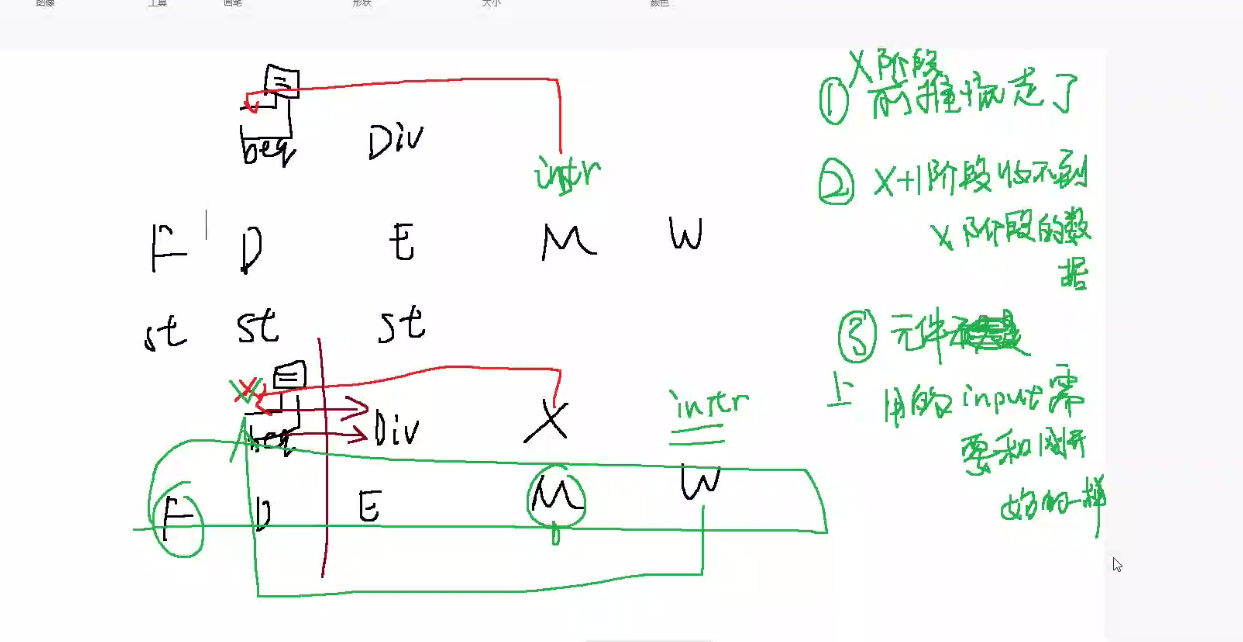
\includegraphics[width=\textwidth]{image/div.png}
        \caption{错误原因}
        \label{div}
    \end{figure}
    \item 修正效果:在陈泱宇学长的指导下,修正有两种方案,第一种是直接修改div的stall为全周期stall,第二种是修改div模块,在里面添加一个reg,用来存放第一个周期传进来的除数和被除数,这样最后一个周期就不会因为op\_data改变而结果出错。我们采用了第二种方法。
    \item 归纳总结:此错误属于时钟同步问题,在添加组件的时候应仔细考虑时钟的影响。
\end{enumerate}

\subsubsection{错误3}
\begin{enumerate}[(1)]
    \item 错误现象:lb指令本来应该改第二个字节,但是却改了第四个字节。
    \item 分析定位过程:vivado仿真得到的错误信息中,与正确答案的第二个和第四个字节不一样,并且修改写入的数据之后,仍然是第二位和第四位不一样。
    \item 错误原因:类sram接口的地址写是由data\_size和data\_waddr同时控制的,我们传出的data\_waddr永远最后两位是2'b00。
    \item 修正效果:传入正确的data\_waddr后,lb指令可以正常运作。
    \item 归纳总结:对类sram接口的理解不够透彻。
\end{enumerate}

\subsubsection{错误4}
\begin{enumerate}[(1)]
    \item 错误现象:从某个时间点开始,一直stall,永远也不停。
    \item 分析定位过程:在跑功能测试的时候,地址永远卡在了0xbfc006d8,查看波形图发现是data\_req发出了请求,并且进行了地址握手,但是永远也等不到它的数据握手。
    \item 错误原因:mycpu\_top模块往mips里面传时钟的时候,没有取反,导致axi接口没有接收到data\_req。
    \item 修正效果:对mycpu\_top传给mips的时钟取反。
    \item 归纳总结:修改文件后,没有全面考虑,导致某些信号没有修改到。
\end{enumerate}

\subsubsection{错误5}
\begin{enumerate}[(1)]
    \item 错误现象:有一个pc在取指阶段没有发出inst\_req请求。
    \item 分析定位过程:查看波形图,发现该pc没有发出inst\_req请求,且发现i\_sram\_to\_sram\_like中的状态机一直处于数据握手ok的状态,发现这个ok是因为d\_stall是置位的,导致数据握手状态没变。
    \item 错误原因:在上升沿的时候,i\_stall变成了0,在下降沿的时候,d\_stall变成了1,导致在下一个上升沿的时候,状态机不会变为空闲状态。
    \item 修正效果:首先考虑了将d\_stall与X\_sram\_to\_sram\_like同步,但是发现实现上可能会导致无法综合的问题。于是考虑将所有组件全部与流水线同步,这样做不仅可以解决上述问题,还可以提升整个mips的性能。
    \item 归纳总结:此错误属于时钟同步问题,在添加组件的时候应仔细考虑时钟的影响。
\end{enumerate}

\subsubsection{错误6}
\begin{enumerate}[(1)]
    \item 错误现象:修改全时钟同步之后,cp0处理int中断时,写入的epc提前了一周期。
    \item 分析定位过程:首先根据错误提示的指令地址查看test.S文件中的对应指令,发现是mfc0 v0,cp0\_epc,这个是把epc取出来的意思,我们发现此处的epc和ref中的epc差了4,于是我们定位到上次发生例外的地方,观察其波形图。发现是mtc0向cp0中写入了一个int中断,写入的一瞬间,exception就发生了, 但是此时i\_stall也是置位的,因此发生错误的那一条指令并没有流入Mem阶段, 导致cp0没有正确把中断指令的地址读到epc中。因此找到了原因。
    \item 错误原因:mtc0向cp0中写入了一个int中断,写入的一瞬间,exception就发生了, 但是此时i\_stall也是置位的,因此发生错误的那一条指令并没有流入Mem阶段, 导致cp0没有正确把中断指令的地址读到epc中。
    \item 修正效果:向cp0传入一个stallM,使得其一同stall,在i\_stall结束后,再把mtc0的数据写进cp0,这样就可以正常的让cp0接收到正确的mtc0地址。
    \item 归纳总结:此错误属于时钟同步问题,在添加组件的时候应仔细考虑时钟的影响。
\end{enumerate}